\documentclass{standalone}
\usepackage{chez}

\begin{document}
\chapter{November 20, 2020}
\subsection{Geometric intuition of Poincar\'e duality}
Consider the torus \(T^2\) with the two standard loops:
\begin{center}
  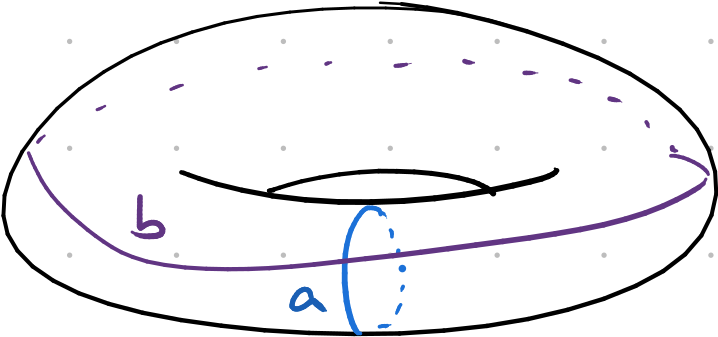
\includegraphics[width=0.27\textwidth]{18_905-201120-1.png}
\end{center}
The loops \(a\) and \(b\) are geometric pictures of cycles
representing generators of \(H_q(T; \FF_2) \iso \FF_2\fgen{a,b}\).

\begin{center}
  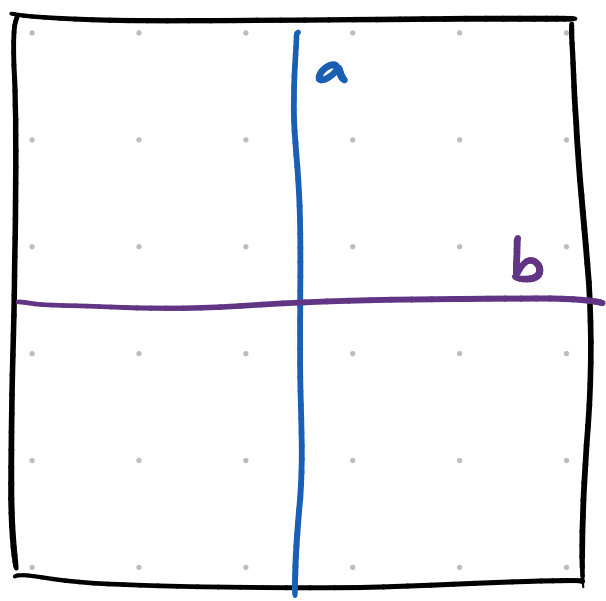
\includegraphics[width=0.18\textwidth]{18_905-201120-2.png}
  \qquad
  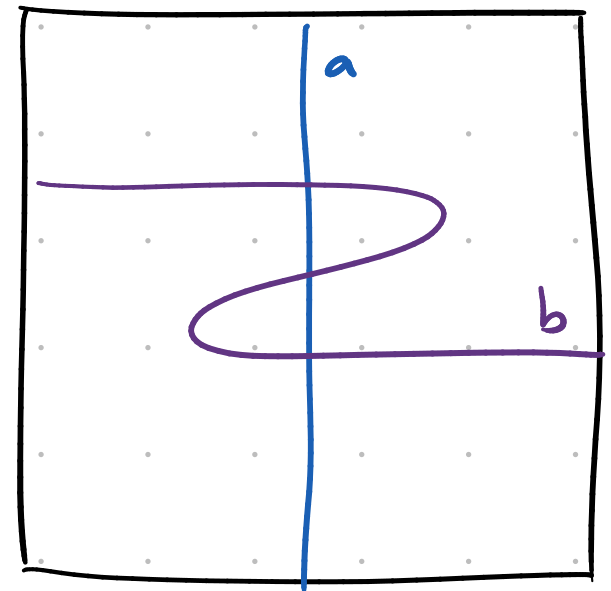
\includegraphics[width=0.18\textwidth]{18_905-201120-3.png}
\end{center}
How many times do \(a\) and \(b\) intersect modulo \(2\)?
No matter how we deform \(a\) and \(b\),
they will intersect an odd number of times.

In very special configurations, they intersect an even number of times.
\begin{center}
  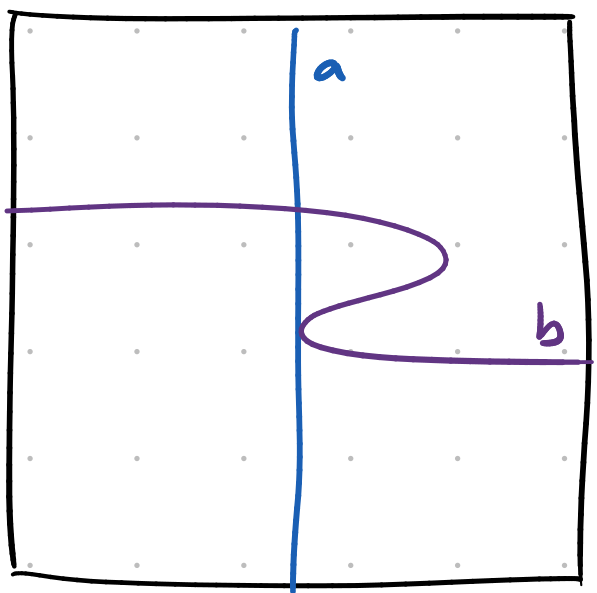
\includegraphics[width=0.18\textwidth]{18_905-201120-4.png}
\end{center}
However, this situation is unstable, i.e.\ deforming \(a\) or \(b\) slightly
will return to an odd number of intersections.

In a class on smooth manifolds, one could prove that the first two pictures
involve \vocab{transverse} interactions, while the last one involves
not transverse interactions.
In order to do this, we would need to go into smooth geometry,
where we can talk about tangent lines.
However, we can use the cup product to talk about these intersections.
In particular, this is a purely topological structure
that does not care about geometry.

We can ask stranger things such as: How many times does \(a\) intersect \(a\)?
We should think about this by thinking about \(a\) as a generic representative
for its homology.
\begin{center}
  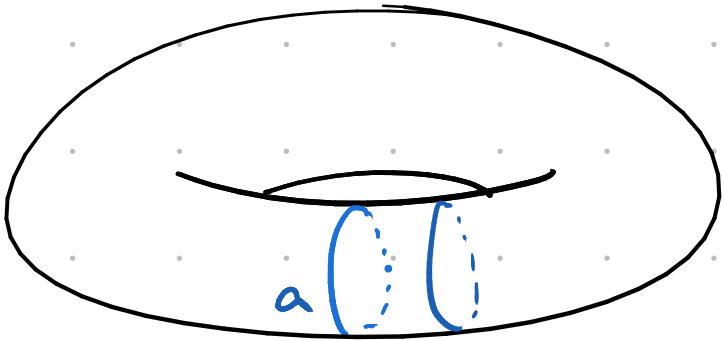
\includegraphics[width=0.2\textwidth]{18_905-201120-5.png}
  \qquad
  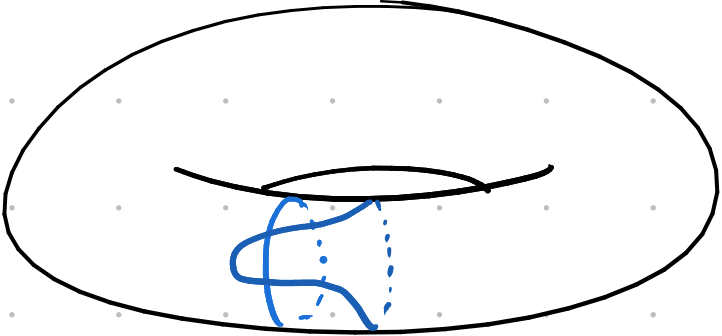
\includegraphics[width=0.2\textwidth]{18_905-201120-6.png}
\end{center}
We can see that generically, \(a\) will intersect \(a\)
an even number of times.

We can define an \(\FF_2\)-module homomorphism
\[
  f_a \colon H_1(R; \FF_2) \iso \FF_2\fgen{a, b} \to \FF_2
\]
which sends \(a \mapsto 0\) and \(b \mapsto 1\),
i.e.\ it counts the number of intersections with \(a\) modulo \(2\).

Using the isomorphism
\[
  H^1(T; \FF_2)
    \iso \ul\Hom_{\FF_2\text{-}\cat{mod}}(H_1(T, \FF_2), \FF_2), % chktex 35
\]
we get that \(f_a\) represents a class in \(H^1(T; \FF_2)\),
which is the \vocab{Poincar\'e dual} of \(a\).


In general, suppose \(M\) is a compact \(n\)-dimensional manifold
where \(p\) and \(q\) are integers such that \(p + q = n\).
If we fix a cycle \(a \in H_p(M; \FF_2)\),
this represents a \(p\)-dimensional submanifold of \(M\).
For any \(b \in H_q(M; \FF_2)\),
\(a\) and \(b\) will intersect at some number
of points, since the dimensions are complementary.
It turns out that the number of points modulo \(2\) is independent
of the generic geometric representatives we chose for \(a\) and \(b\).

Overall, if we fix \(a \in H_p(M; \FF_2)\) and vary \(b \in H_q(M; \FF_2)\),
we get a function
\[
  f_a \colon H_q(M; \FF_2) \to \FF_2,
\]
which can be viewed as a class in \(H^q(M; \FF_2)\).
The Poincar\'e duality theorem says that this defines an isomorphism
\begin{align*}
  H_p(M; \FF_2) &\iso H^q(M; \FF_2) \\[-1ex]
    a &\mapsto f_a.
\end{align*}
In particular, this states a cycle, modulo boundaries,
is determined by the number of times it intersects all other cycles
in complementary dimension.


Last time, we had the perfect pairing
\begin{align*}
  P \colon& H^q(X; \FF_2) \otimes H^p(X; \FF_2) \to \FF_2 \\[-1ex]
    & u \otimes v \mapsto \angles{uv, [M]}
\end{align*}
which induces an isomorphism
\begin{align*}
  H^q(M; \FF_2)
    &\iso \ul\Hom_{\FF_2\text{-}\cat{mod}}(H^p(X; \FF_2), \FF_2) \\ % chktex 35
    &\iso H_p(X; \FF_2).
\end{align*}

\begin{claim}
  These two isomorphisms are equivalent.
\end{claim}

\begin{remark}
  The fundamental class \([M] \in H_n(M; \FF_2)\) is Poincar\'e dual to
  \(1 \in H^0(M; \FF_2) \subseteq H^*(M; \FF_2)\),
  the function that takes every path component to \(1\).
  Geometrically, this is the class that covers the whole manifold
  if we think about intersections.
\end{remark}

There is also a version of Poincar\'e duality with integer coefficients,
but it's more complicated and only works for oriented manifold.
The idea is as follows:

Consider the torus \(T^2\), which will be oriented,
and the loops \(a\) and \(b\) from before,
where they intersect three times and we give them directions.
In particular, consider the diagram with three intersections,
and zoom into the three intersections.
\begin{center}
  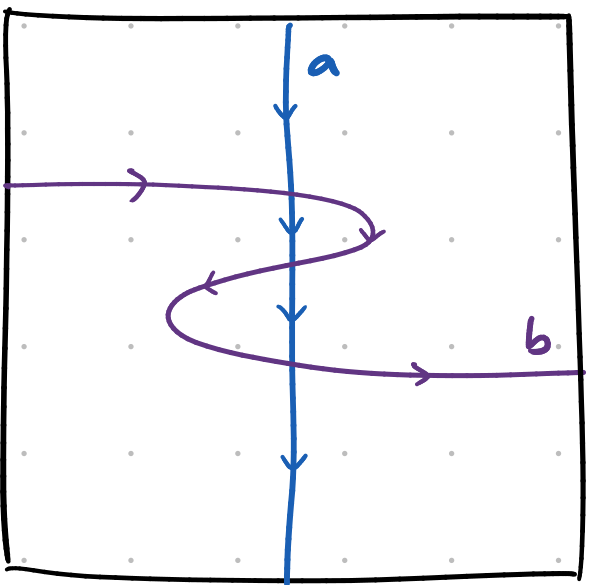
\includegraphics[width=0.22\textwidth, align=c]{18_905-201120-7.png}
  \qquad
  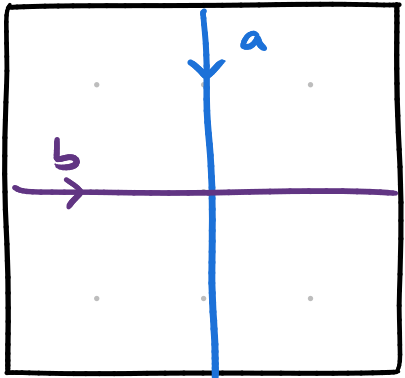
\includegraphics[width=0.18\textwidth, align=c]{18_905-201120-8.png}
  \qquad
  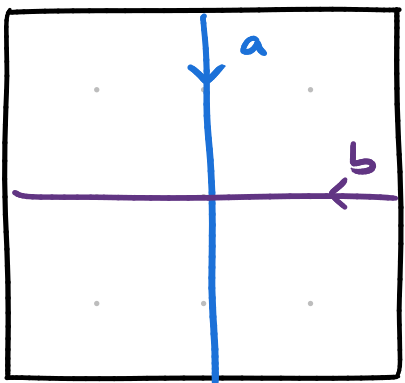
\includegraphics[width=0.18\textwidth, align=c]{18_905-201120-9.png}
  \qquad
  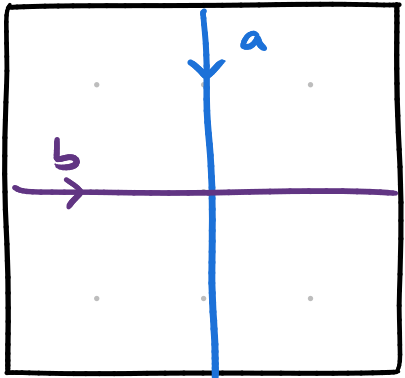
\includegraphics[width=0.18\textwidth, align=c]{18_905-201120-8.png}
\end{center}
The idea is that the last two diagrams differ by a reflection,
and when we count intersections, we do a signed count,
where a reflection introduces a minus sign.
Therefore, the last two diagrams cancel each other out,
and there is only one signed intersection.

However, this only works for oriented manifolds because
for nonoriented manifolds, going around in a loop might cause
the diagrams to be inconsistent, i.e.\ they will become reflected.

\section{More applications of Poincar\'e duality}
Last time, we computed \(H^*(\RP^2; \FF_2) \iso \FF_2[a]/a^3\).
But more generally, we can compute \(H^*(\RP^n; \FF_2)\).
\begin{example}[\(H^*(\RP^3; \FF_2)\)]
  As a graded vector space, we have
  \[
    H^*(\RP^3; \FF_2)
      \iso \underbracket{\FF_2\fgen{1}}_{\deg 0} \oplus
           \underbracket{\FF_2\fgen{a}}_{\deg 1} \oplus
           \underbracket{\FF_2\fgen{b}}_{\deg 2} \oplus
           \underbracket{\FF_2\fgen{c}}_{\deg 3}.
  \]
  In particular, we have the perfect pairing
  \[
    P \colon
      H^1(\RP^2) \otimes_{\FF_2} H^2(\RP^2) \iso \FF_2\fgen{a \otimes b}
      \to \FF_2
  \]
  where \(P(a \otimes b) = \angles{ab, [\RP^3]}\).
  In particular, this is a nontrivial map \(\FF_2 \to \FF_2\),
  so \(ab \neq 0\), and furthermore \(ab = c\).

  We can completely determine \(H^*(\RP^n; \FF_2) \iso \FF_2[a]/a^{n+1}\)
  where \(\size a = 1\).
\end{example}


\begin{theorem}[Borsuk-Ulam]
  Let \(f \colon S^n \to \RR^n\) be a continuous function.
  There exists \(x \in S^n\) such that \(f(x) = f(-x)\).
\end{theorem}
\begin{example}
  At any moment in time, some antipodal pair of points on Earth
  share the same temperature and air pressure.
\end{example}
\begin{proof}
  Suppose no such \(x\) exists.
  Consider
  \begin{align*}
    g \colon& S^n \to S^{n-1} \\[-1ex]
      & x \mapsto \frac{f(x) - f(-x)}{\abs{f(x) - f(-x)}}.
  \end{align*}
  This is well defined because the denominator is never zero.
  Note that \(g(-x) = -g(x)\).
  Hence, there is a continuous map \(\bar g \colon \RP^n \to \RP^{n-1}\)
  induced by \(g\).

  We claim that the map
  \[
    H_1(\bar g; \FF_2) \colon H_1(\RP^n; \FF_2) \iso \FF_2
                            \to H_1(\RP^{n-1}; \FF_2) \iso \FF_2
  \]
is nontrivial.
Consider the path in \(S^n\) going from the north pole to the south pole.
Upon projection to \(\RP^n\), this becomes a cycle that generates
\(H_1(\RP^n; \FF_2)\).
Mapping under \(\bar g\) gives a nontrivial element of
\(H_1(\RP^{n-1}; \FF_2)\).

We now proceed with the remainder of the proof.
By Poincar\'e duality, we have that \(H^1(\bar g; \FF_2)\) is nontrivial.
In particular, the following map must satisfy
\begin{align*}
  H^*(\bar g; \FF_2) \colon& H^*(\RP^{n-1}; \FF_2) \to
                             H^*(\RP^{n}; \FF_2) \\[-1ex]
    \colon& \FF_2[a]/a^n \to \FF_2[a]a^{n+!} \\[-1ex]
    & a \mapsto a,
\end{align*}
but there is no such ring map, which is a contradiction.
\end{proof}


\end{document}
